\chapter{Technical}
	In this chapter, we explain our motivating scenario in more detail, explore the sensor hardware that we researched and outline the results of experiments we undertook in the Malaysian rainforest. As highlighted in Section \ref{int:mot}, we have been working with Cardiff University School of Bioscience to design and deploy a WSN that utilises local knowledge, using an area of rainforest in Malaysia owned by the Sabah Wildlife Department, called Danau Girang.

The structure of this chapter is as follows. Section \ref{tech:motiv} explains what we aimed to deploy in Danau Girang and what our considerations were. Secion \ref{tech:hw} introduces sensor hardware that is in use today and details the choices we made. Section \ref{tech:wireless} details the transmission medium choices we tried and also shows the results of experiments performed in both the UK and Malaysia. Finally, Section \ref{tech:conc} summarises our findings and explains the choices we made for the sensor nodes we used in DG. 

\section{Danau Girang}
	Based in Sabah, Malaysia, Danau Girang is a field centre located in Lot 6 of the Lower Kinabatangan Wildlife Sanctuary (LKWS), surrounded by secondary rainforest that had been logged up until the 1970s. Experiencing typical wet and dry seasons, the LKWS can receive more than 500mm of rainfall during the rainy season, dropping to lows of around 150mm during the dry seasons \cite{Walsh2009}, and up to 100\% humidity all year round. 

Danau Girang is uniquely situated in a rainforest corridor that joins two areas of rainforest together, with the corridor surrounded by palm oil fields on each side. Because of this, animals use the corridor to move between the rainforest regions and some use it to enter the palm oil plantation for new feeding grounds. This gives Danau Girang insight into the movement patterns of these animals in the corridor as well as in the rainforest itself, with a wide variety of species that are not commonly seen in other tropical regions of the world. Due to the remote nature of the centre, power is provided by a set of diesel generators which, typically, provide power from 10 am to 1 pm and 5pm to 11pm daily. Wireless Internet access is provided by satellite with speeds comparable to that of 56k, although the upload speeds are considerably faster than downloads.

As outlined in Section \ref{int:mot}, the corridor monitoring programme is a scheme that has been in place for more than five years to use wildlife cameras to track the movement of animals through the corridor and to capture species that are rare or unique to South-East Asia, such as the Bornean Clouded Leopard or Sun Bear. Currently, the use of Reconyx Hyperfire HC500 cameras are being used \cite{Reconyx}. These are standalone cameras that store a pre-defined set of images to an SD card on each trigger, which is triggered by an infrared (IR) motion sensor when the beam is broken. 

Images must be collected manually every two weeks from the cameras and the batteries are changed at that point as well, although a typical charge should last three months. The cameras are equipped with watertight casing but, due to the humidity and the opening of the cameras every 2 weeks, silica gel is used to prevent moisture inside the camera. We believe that humidity also reduces the battery life, as the charge drops from three months to around three weeks within the first few months of usage. However, the lack of constant power availability could also negatively impact the charge cycles of the batteries when at the field centre, reducing their capacity. Each unit is secured to a tree and more dangerous sites, such as known elephant paths, have protective cases as well. 

In 2010, twenty cameras were deployed for six month periods and then relocated based on the needs of the projects at that time. As of 2013, there are now ninety 	with a view to expand and dozens of projects within the field centre use the images gathered from these cameras. Initially, it was the job of visiting research students to collect the images but, since the number of deployed cameras has grown, full-time staff have been taken on to maintain them.

Our belief is that we can use the LKWS, and the locations of the existing cameras, to deploy a WSN that uses local knowledge gained from the researchers at DG to automate the collection of images, improve the battery life by not exposing the internals of the camera to the elements so often and, most important, prioritise the flow of data through the network by in-network processing. 
	
Annual visits, lasting three weeks, have been made to DG to test out hardware, software and wireless choices, in an effort to optimise the network. These visits have also been used to extract local knowledge from the area and researchers, by semi-structured interviews and watching them work.

\section{Hardware}
	Before any visits were made to DG, meetings with staff members of the field centre were held in order to gain a better understanding of the environment and the project. This is where we were alerted to the humidity of the region and the fact that the failure rate of the Reconyx cameras has been as high as thirty per cent.

Reconyx cameras have no external interface support and the only way to access the images is through the removable SD card, because of this there is no way of attaching external sensor hardware to the existing cameras. In-network processing is an important requirement for our WSN and this did limit our choices to nodes that are computationally capable than more common sensors, such as the IMote 2 \cite{Nachman2008}.

In this section, we detail our research into suitable sensor hardware that met the following requirements:
\begin{enumerate}
	\item Able to perform processing of images and metadata
	\item Common interface availability (Serial, USB)
	\item Wireless enabled
	\item Battery-powered
	\item Expandable memory
\end{enumerate}
This section also details the modifications we made to the devices in order to ensure they would survive in a humid environment.

\subsection{Pandaboard}

Texas Instruments supported the development of a reference Single Board Computer (SBC) that had specs similar to that of a modern smartphone and was capable of running desktop Linux, known as the Pandaboard \cite{instruments2012pandaboard}. A dual core 1GhZ ARM processor with 1GB of RAM, support for external storage, expansion ports, USB, Wi-Fi and Bluetooth in a board the size of two credit cards can be a powerful addition to a data heavy WSN, especially one that deals with images.

There is no mention of Pandaboards in the literature being used in WSNs but, the low power of the system and advanced capabilities, make it suitable for processing and transmitting data simultaneously. 
	
\subsection{IGEP v2}

The IGEP v2 is another ARM based SBC that uses a 1GhZ single core processor with 512MB RAM and similar connectivity features to the Pandaboard, but around half the size. This does result in a reduced power draw and the device is still capable of running desktop Linux.

Due to the smaller size, and easier commercial availability, the IGEP has been used as a sensor node to record, process and send readings from multiple devices, such as air temperature, GPS and oxygen saturation as part of environmental monitoring \cite{Resch}. In their research, they found that the IGEP achieved 9.1 hours of uptime using a 4000mAH battery, a capacity used in many modern smartphones.

\subsection{Waspmote}
The Waspmote is a general purpose sensing board that is designed to allow plug-and-play connectivity for multiple sensor modules. The node can be programmed with C++, using the prepackaged SDK. The processing power is not comparable to the more powerful SBCs, but the 600mAh battery is reported to be three months and the size is much smaller \cite{Lib}.

One of the benefits of the Waspmote is that they are commercially available with an actively maintained programming environment.

\section{Transmission Medium}
	In this section, we explain the experiments we carried out to test the performance of different transmission media in the UK as well as the Malaysian rainforest. While range is the most important feature, a data rate that can handle hundreds of images a day is also a necessity.

\subsection{Wi-Fi}\label{tech:wifirange}
Wi-Fi was already available on our initial test platforms and the high data rate made it suitable for sending a large volume of images in a short period. We knew that current cameras deployed in DG were up to 1km apart and we did not expect to cover that range completely, but were did anticipate that coverage with intermediate nodes.

Research, outlined in Section \ref{bg:trans}, showed us that the rainforest could reduce the range by up to 78\% and the ideal maximum range of 2.4GhZ Wi-Fi is 100m \cite{Dhawan2007}. 

We tested Wi-Fi range using two IGEP boards, powered by 4 D Cell batteries and running a lightweight Linux operating system.	The IGEP nodes we used did not have any additional hardware and the nodes were tested without the use of an external antenna. A Java application was written to periodically scan for available networks and store those results in a text file. One IGEP board was set as the base station and attached to a tree, at the same height it would be if it was attached to a camera, and another was walked to specified points around the base station at defined locations. These locations were chosen to include as many distances as possible and as many different forms of obstacle between the searching node and the base station, such as: line of sight (LOS), medium vegetation or thick trees.
			
This experiment was run in a wooded area in the UK and in the rainforest at DG. The specified maximum range of 802.11g is 120m. When considering attenuation and obstacles we were expecting the signal to be reduced by up to 50\% in the UK. However, we found that we received a maximum range of 30m, with LOS. Figure \ref{cardiffsnr} shows the results we experienced, while testing in Cardiff, some of the drops in signal can be attributed to dense foliage and readings that were not LOS, but a maximum range of 31m, with an SNR of 29.5 dBm, is less than we expected, as the UK does not experience high humidity often.
			
			\begin{figure}[!t]
			\centering
			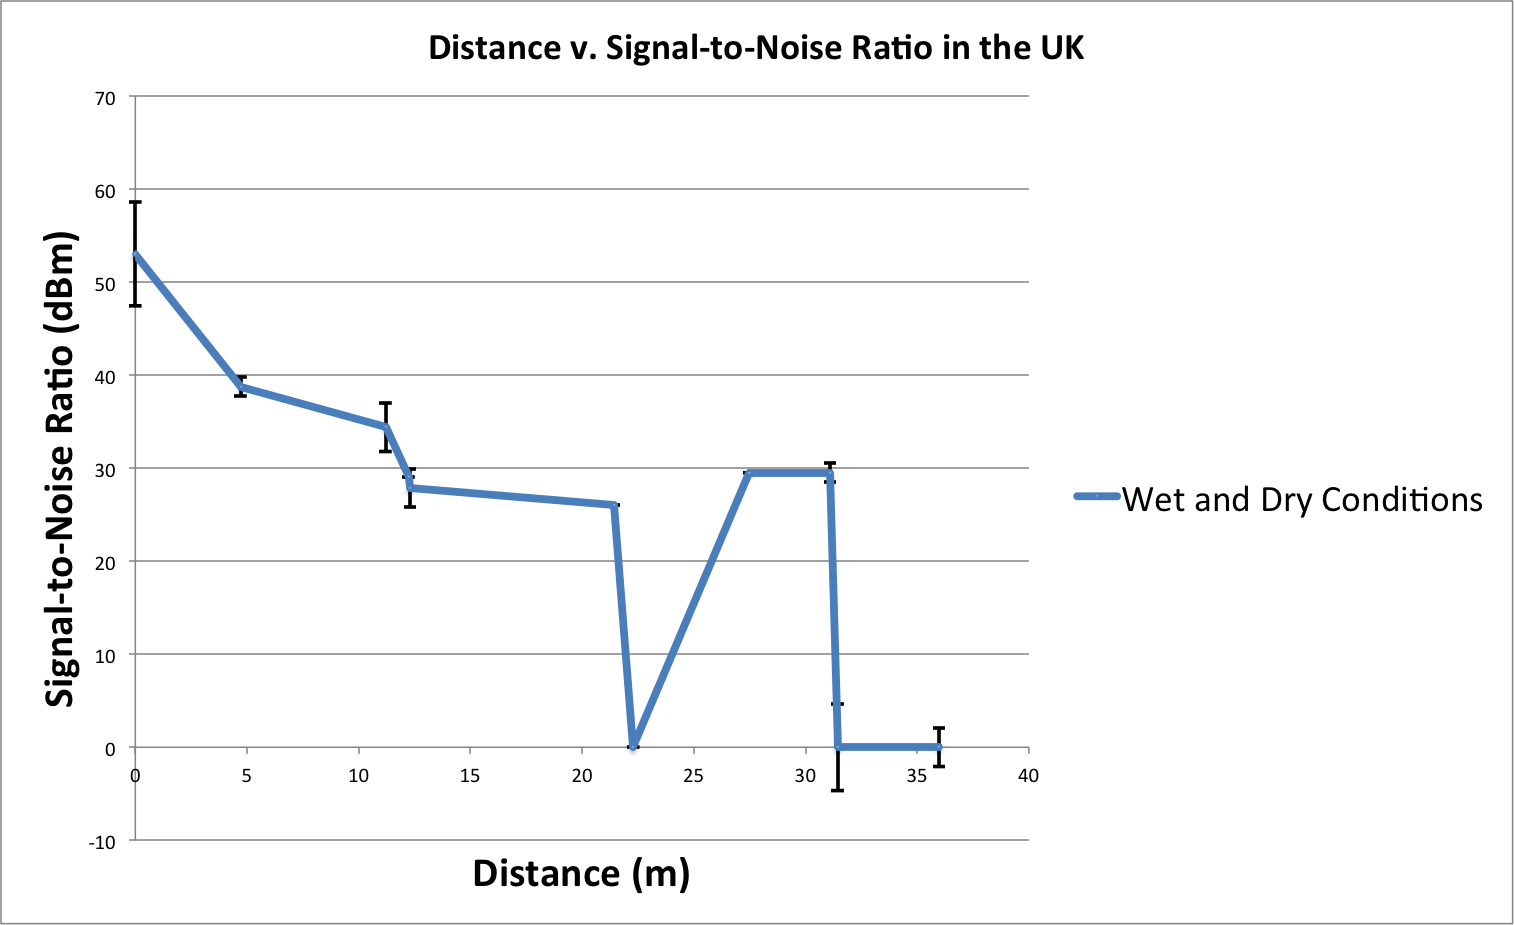
\includegraphics[width=0.45\textwidth]{Chap3/figures/bp_snr.png}
			\caption{Signal-to-Noise Ratio for Wi-Fi in UK Woodland}
			\label{cardiffsnr}
			\end{figure}
			
	The graph does show a drop at 22m, this was due to the dense foliage that restricted the LOS between the base station and the receiving node, with five runs of this test we observed the same results. The primary aim of this experiment was to prove the viability of Wi-Fi and to to ensure our application functioned as intended, which it did. Further experiments could have been run to remove the anomaly but the results of the experiments in Danau Girang were the focus.
		 
	Despite the poor range from the tests in the UK, it was consistent with other studies reporting signal degradation of up to 78\% in areas with moderate foliage. We visited Danau Girang in 2011 to gather the requirements of the network and ensure the hardware is able to survive the humidity. Range experiments were run in the rainforest to see if a more humid environment impacts range any further, Figure \ref{malaysiasnr} shows this.
			
			\begin{figure}[!t]
			\centering
			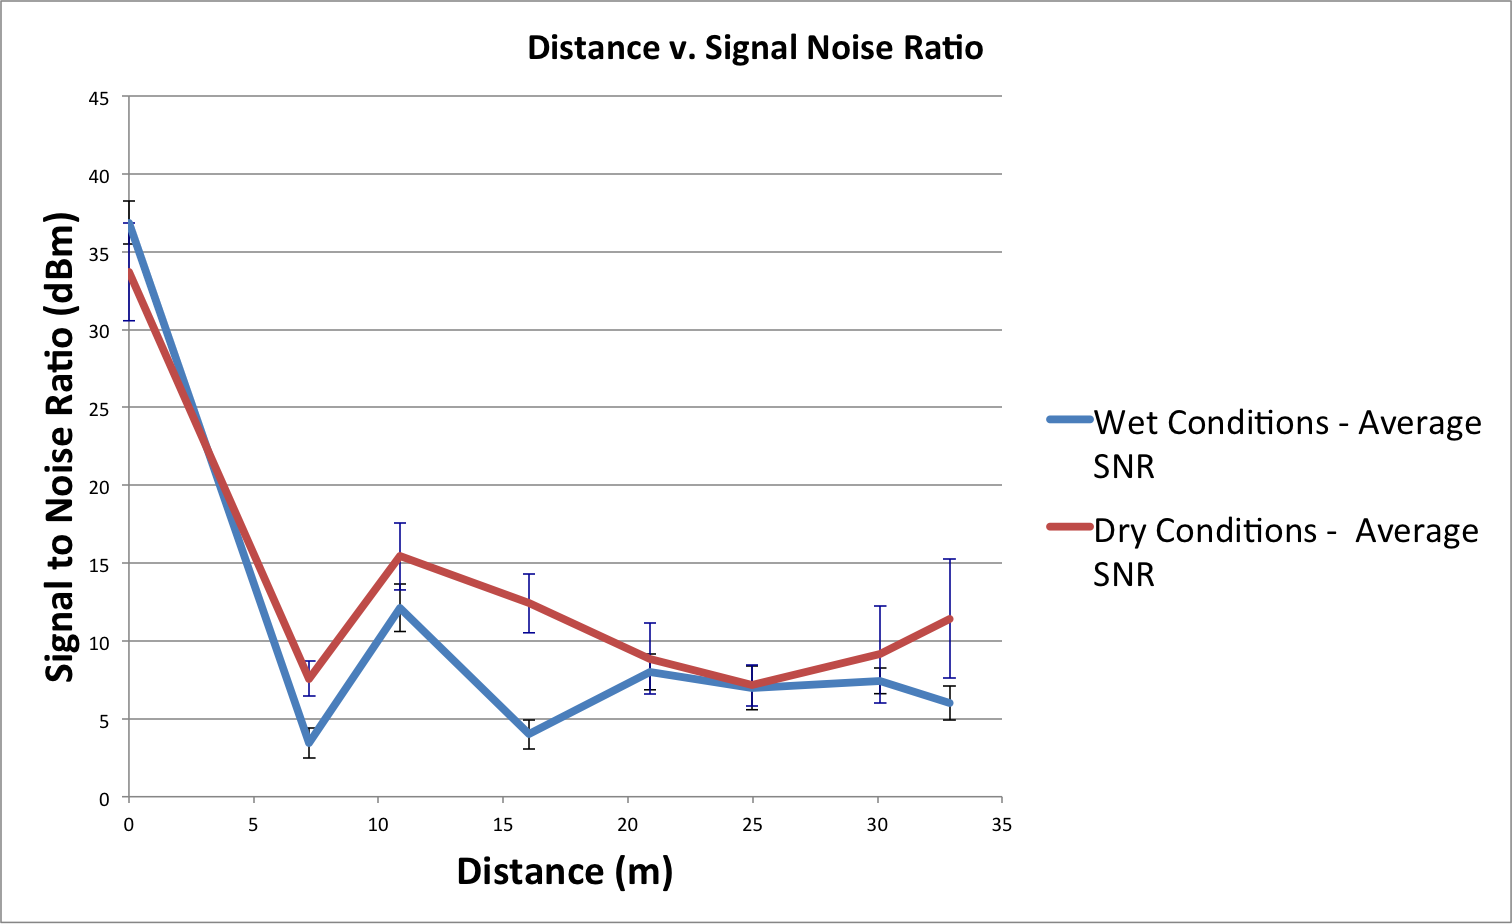
\includegraphics[width=0.45\textwidth]{Chap3/figures/dg_snr.png}
			\caption{Signal-to-Noise Ratio for Wi-Fi in Malaysian Rainforest}
			\label{malaysiasnr}
			\end{figure}
						
			Comparing figures \ref{cardiffsnr} and \ref{malaysiasnr} shows that the maximum distance to receive a signal is approximately the same in Malaysia as it is in the UK.  There are more signal drops but this seems to be due to denser foliage blocking the line of sight. However, it does suggest that the humid environment of the rainforest does not have a significant impact on the received signal. It is clear that the denser rainforest does impact the signal-to-noise ratio in a much shorter distance from the base station but a link is still made, allowing for a successful transmission of data.
			
Due to the poor results of these experiments we researched alternative methods to increase the range without impacting the environment the network is to be deployed in. We considered using intermediate nodes, not attached to cameras, to account for the lack of range but, because some cameras can be up to 1km apart, we would need more than 30 nodes to create a connection between two locations.
			
We also researched wireless technologies that are more common in sensor networks. This does mean that the data rate is not as high as Wi-Fi and error correction in packet streams is not always as robust, but it is more suited to sensor networks, using less power and providing longer range.
			
Finally, we considered using the researchers or animals at Danau Girang, as `data mules', creating temporary links between nodes while they are in the forest. However, the trip to Danau Girang yielded the information that researchers generally do not cover those distances in the forest and data delivery would be sporadic.
			
Although the range of Wi-Fi is poor, for our requirements, in both Malaysia and the UK, it did show that the results we experience in the UK are very similar to the results in Malaysia. This means that tests run in the UK should be indicative of what we can expect in Danau Girang.

\subsection{Digimesh}
		Due to the poor range results of Wi-Fi, we created a second prototype of the network, using Digimesh. Digimesh is a proprietary wireless protocol, based on the 802.15.4 standard and designed for devices with limited power. Using the same frequency as Wi-Fi, Digimesh has been reported to provide 7km of range, with a data rate of 250kbps.
		
In our prototype implementation, we are using Waspmote sensor boards \cite{Waspmote}, a general purpose node that is capable of transmitting through various communication mediums. Our Waspmotes are provided with Digimesh modules and a 2GB SD card to store sensed data.
		
When testing the range of the Waspmotes, we followed a similar method to that which is outlined in Section \ref{sec:wifirange}. One board is in a fixed location and running a C++ application to poll for nodes in the network, once a node is found it sends a message to the node every 10 seconds. The second board is set to scan the network and receive packets as soon as a base node is found, this node is then moved to different locations.
			
The receiving node prints out variables related to the received packet, such as: RSSI, source MAC address and packet ID. However, not all packets are received so the RSSI can display 0 if there are errors reading or if packet collision occurs. We found this to affect the results and have just used the two nodes to identify the maximum distance they can be apart, while maintaining a stable connection.
					
Initial experiments were run in a moderately vegetated area in the UK which yielded 497m of range. Limitations with buildings preventing us from testing any further but the signal strength still proved to be strong.
			
The initial results for the range tests proved positive and Digimesh does seem to be a viable solution to account for the lack of range when using Wi-Fi. As the frequency is the same as 802.11g, thus licensing it for worldwide use, we expected similar results in Danau Girang..
						
Experiments were run in 2 areas of the rainforest around Danau Girang and the results yielded were not the same as we experienced in the UK, and thick vegetation proved to have a significant impact on the range, reducing it by almost 50\%.
			
In more open areas of the rainforest, we achieved 199m on average, more dense regions of the forest reduced this to 102m on average. While these results are not as high as we achieved in the UK, they are still suitable to use Digimesh in the deployment of a WSN.

\subsection{Adapting for Harsh Environments}
	All of the hardware that we used for experiments had their components exposed and would have become compromised if moisture came in contact with them. To protect them from this, we used waterproof cases with a protective foam inside, known as Pelican cases, to keep the nodes watertight, but still allowing airflow, shown in Figure \ref{tech:pelican}.
	External antenna can be fed through the lip of the case, using thin cable, ensuring that the range of the transmissions is not affected by the case. 

			\begin{figure}[!t]
			\centering
			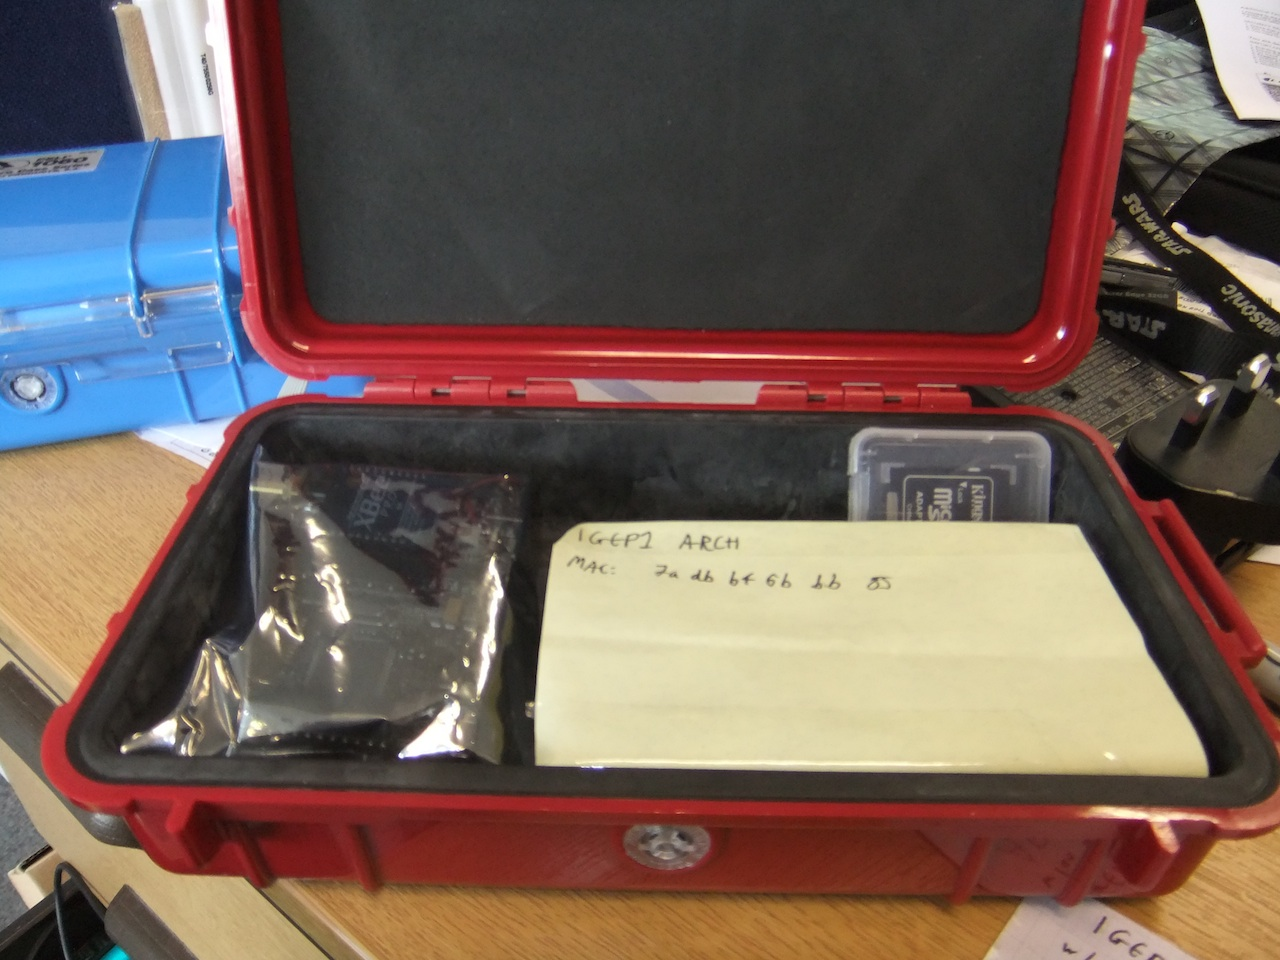
\includegraphics[width=0.45\textwidth]{Chap3/figures/pelican}
			\caption{Pelican Waterproof Case}
			\label{tech:pelican}
			\end{figure}

\subsection{Commercial Solution}
	Using commercial hardware, either bespoke for sensing or more general-purpose, our experiments showed that the range experienced in practice is much less than what is expected. Due to the lack of available interfaces available on the Reconyx cameras in use at Danau Girang, any sensor node would have to be connected to an external camera.
	Because of these factors, we began to look into commercial solutions that combined wildlife cameras with wireless transmission capabilities. 

\section{Summary}
	In this chapter, we have shown the current hardware choices available for more computationally capable sensors and detailed our experimental results on how rainforest environments impact wireless transmissions. Although technologies, such as Wi-Fi, provide a high data rate, their range is limited and not suitable for sparse sensor networks; especially in a humid environment.
	Newer technologies, designed for long-range communication in sensor networks, are becoming increasingly more viable and, while they do have lower data rates and less robust protocols, they are more suitable for a resource constrained WSN that requires minimal power draw when transmitting. 
	Using general-purpose hardware also means that there is no protection against water, humidity and animal or human intervention. We have adapted existing waterproof cases to suit our needs and two week deployments have shown that they are able to prevent any moisture from entering the case.
	 